\documentclass[a4paper,11pt]{ltjsarticle}
\usepackage{graphicx}
\usepackage{luatexja-fontspec}
\usepackage{caption}
\usepackage{amsmath,amssymb,bm,braket}
\usepackage[english]{babel}
\usepackage{multicol}
\usepackage{titlesec}
%\usepackage{gnuplot-lua-tikz}
\usepackage[top=20truemm,bottom=20truemm,left=20truemm,right=20truemm]{geometry}
\usepackage{array}
\usepackage{upgreek}
\usepackage{fancyhdr}
\renewcommand{\refname}{}
\usepackage{listings,jvlisting}
\usepackage{tikz}
\usepackage[thmmarks,amsmath]{ntheorem}
\usepackage[version=3]{mhchem}
\usetikzlibrary{external}
\tikzexternalize
\lstset{
  basicstyle={\ttfamily},
  identifierstyle={\small},
  commentstyle={\smallitshape},
  keywordstyle={\small\bfseries},
  ndkeywordstyle={\small},
  stringstyle={\small\ttfamily},
  frame={tb},
  breaklines=true,
  columns=[l]{fullflexible},
  numbers=left,
  xrightmargin=0pt,
  xleftmargin=3pt,
  numberstyle={\scriptsize},
  stepnumber=1,
  numbersep=1pt,
  lineskip=-0.5ex
}
\captionsetup[figure]{format=plain, labelformat=simple, labelsep=quad,labelfont=bf,name={Fig.}}
\captionsetup[table]{format=plain, labelformat=simple, labelsep=quad,labelfont=bf}
\parindent = 0pt
%[BoldFont=HGSMinchoE]{MSMincho}[BoldFont=HiraMinProN-W6]{HiraMinPro-W3}
\titleformat{\section}{\normalfont\fontsize{9}{10}\bfseries\fontspec{Times New Roman}}{\thesection.}{1em}{}
\usepackage[backend=biber,sorting=none,style=numeric,maxnames=99,minnames=1]{biblatex}
\addbibresource{utility/REFERENCES.bib}
\defbibheading{bibliography}[\refname]{%
  \section*{REFERENCES}%
  \vspace{-7pt}  % ここで空白を調整。お好みの値に変更してください。
}
\newfontfamily\subsectionfont{Times New Roman} % サブセクション用フォント
\titleformat{\subsection}
  {\normalfont\large\bfseries} % サブセクションのフォントを指定
  {\thesubsection}{1em}{}
\renewbibmacro{in:}{}
\renewbibmacro*{journal+issuetitle}{%
  \addcomma\space% カンマとスペースを追加
  \usebibmacro{journal}%
  \setunit*{\addspace}%
  \usebibmacro{volume+number+eid}%
  \setunit{\addspace}%
  \printfield{note}%
  \newunit
}
\renewbibmacro*{volume+number+eid}{
  \printfield{volume}%
  \setunit*{\addnbspace}%
  \printfield{number}%
  \setunit{\addcomma\space}%
  \printfield{eid}
}
\DeclareFieldFormat[article]{volume}{\textbf{#1}}
\DeclareFieldFormat[article]{pages}{#1}
\DeclareFieldFormat{journaltitle}{#1}
\usepackage{hyperref}
\renewenvironment{abstract}{\par\noindent}{\par}
%\pagenumbering{gobble}
\usepackage{docmute}
\usepackage{setspace}
\usepackage{titlesec} % 見出しのカスタマイズ用

% セクションのフォーマットをカスタマイズ
\titleformat{\section}
  {} % フォントサイズとスタイル
  {\Large\bfseries\thesection\ \ }               % 番号の前の内容(空白)
  {0em}            % 番号とタイトルの間の間隔
  {\Large\bfseries}


\theoremstyle{plain}
\theoremheaderfont{\normalfont\bfseries}
\theorembodyfont{\itshape}   % 本文を斜体に
\theoremseparator{.}         % タイトルと本文の区切りを「.」に設定
\newtheorem{definition}{Definition}
\begin{document}
\section{Looped Pipeline Architecture}{
    \ \ \ Many quantum computing platforms are based on a two-dimensional physical layout. We focus on "looped pipelines," \cite{cai2023} which offer the advantages of a three-dimensional lattice while being restricted to two-dimensional space. This architecture leverages qubit shuttling, where qubits are moved around on the chip, enabling long-range interactions between qubits that are far apart. 

    \subsection{Classical Linear Pipeline}{

        \begin{figure}[h]
            \centering
            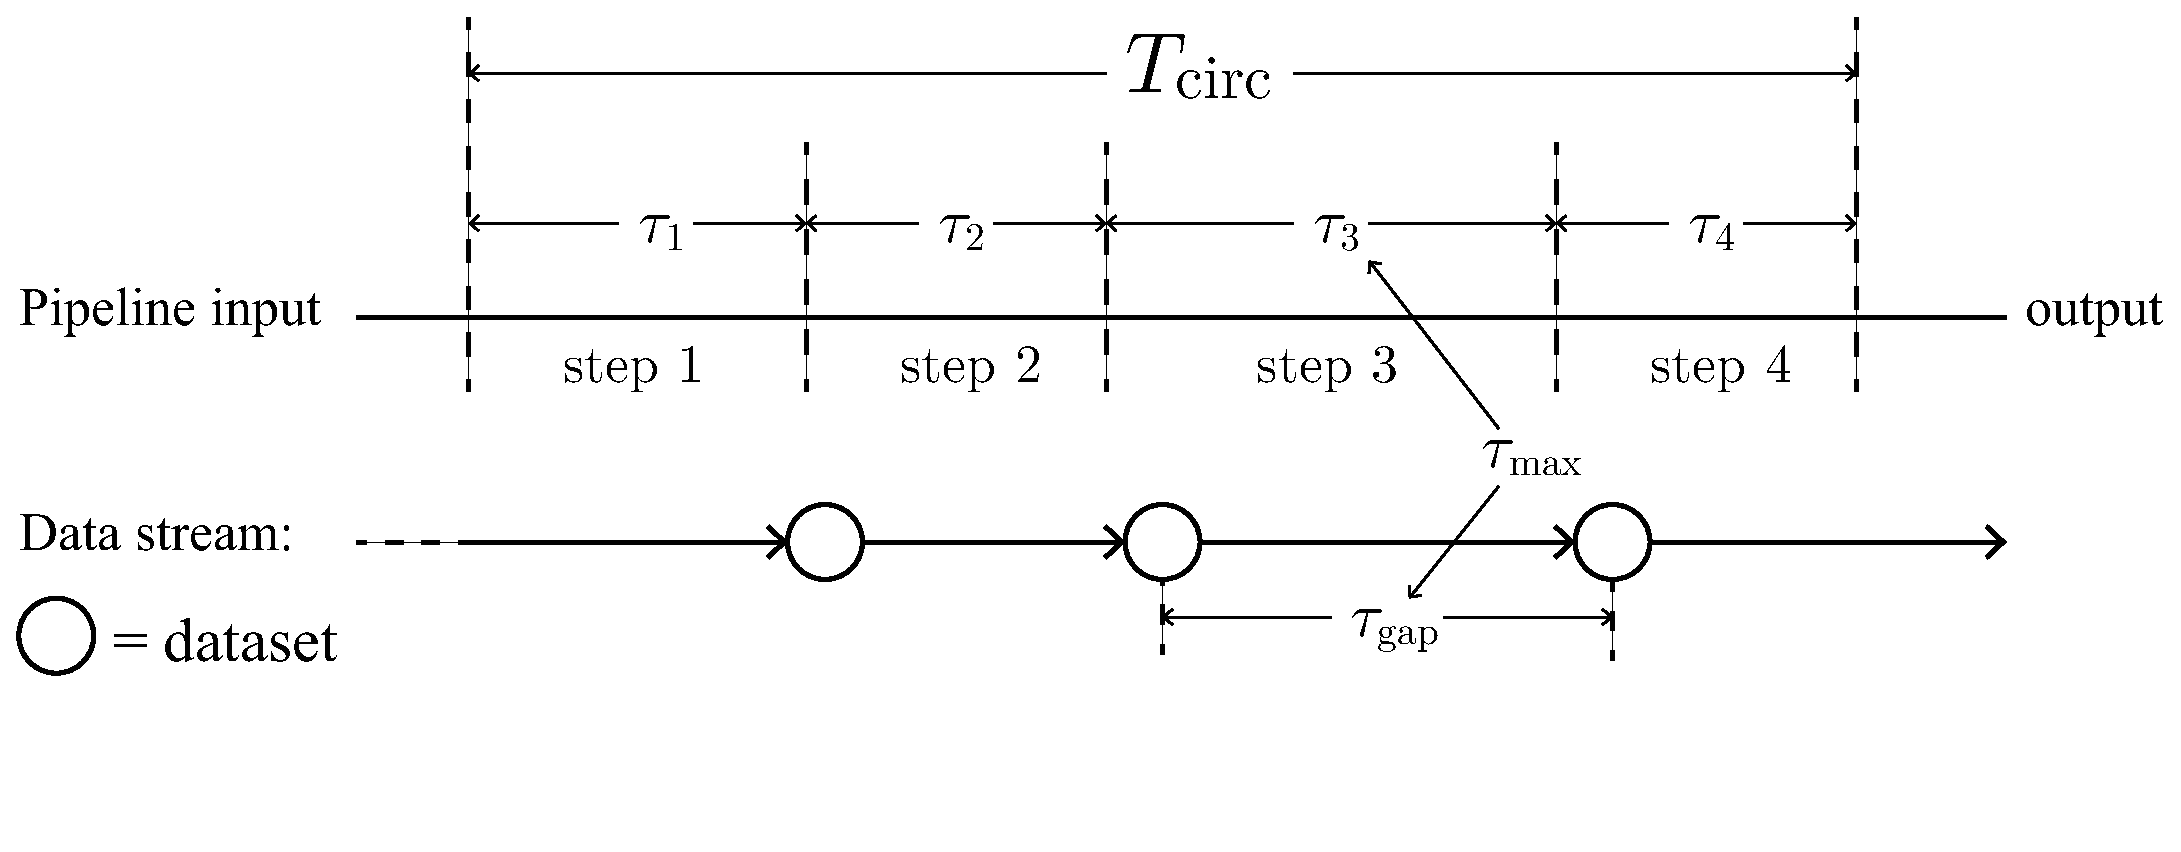
\includegraphics[scale=0.40]{figure/classical_pipeline.eps}
            \vspace{-20pt}\caption{}
            \label{classical_pipeline}
            \vspace{-10pt}
        \end{figure}

        \ \ \ Let us fist introduce "data-processing pipeline," we divide data-processing circuit into multple steps with each step able to operate only one dataset at a time shown in Fig.~\ref{classical_pipeline}. Now intead of inputting second dataset after the processing the first dataset on whole circuit, we input it as soon as finishing the process of the first dataset on step 1, similarly all subseaquent datasets and subseaquent steps. In this way, all data-processing steps can be working on different datasets in parallel, increasing the throughput of the system. this is a concept of pipelining. 
        \ \ \ The processing time of the $m$th step is denoted as $\tau_m$, and suppose there exist $M$ steps in the circuit. Then, the total time $T_{\text{circ}}$ taken for the entire circuit to process one dataset is given by:
        \begin{align}
            T_\text{circ}=\sum_{m=1}^M\tau_m.
        \end{align}
        This is the time required for every dataset without pipelining, and it is also the time required to process the first dataset in pipelining. For the second dataset in pipelining, the additional time required for processing is given by:
        \begin{align}
            \tau_\text{max}=\max_i{\tau_i}.
        \end{align}
        From the second dataset onward, the time required for processing each dataset equals the maximum of $\tau_i$. Hence, the total time for processing the $k$th datasets are given by:
        \begin{align}
            T_\text{pipe}=T_\text{circ}+(k-1)\tau_text{max}.
        \end{align}
        The data stream can flow through the entire pipeline without requiring modifications to the time gap between adjacent datasets or being put on hold at any point along the pipeline.
    }
    \clearpage
    \subsection{Looped Qubit Pipeline}{
        \begin{figure}[h]
            \centering
            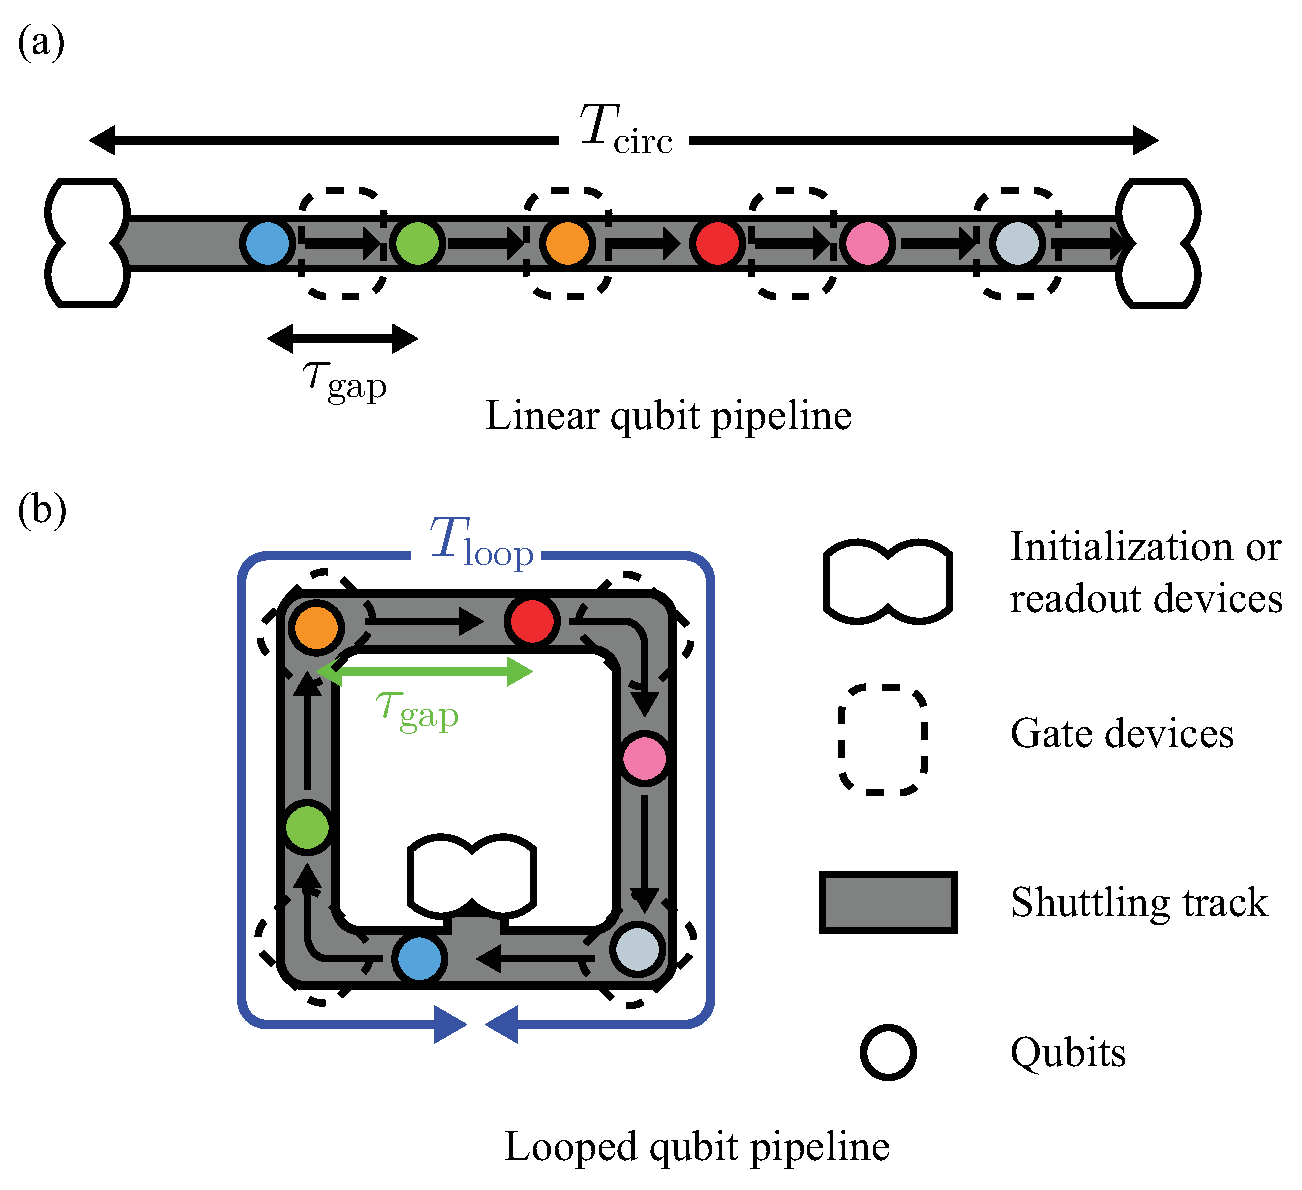
\includegraphics[scale=0.50]{figure/shuttling_track.eps}
            \vspace{0pt}\caption{}
            \label{shuttling_truck}
        \end{figure}
    }
}
\end{document}